\documentclass[11pt]{article}
\title{Agent Reliability at the External-Effect Boundary: Conditional Evaluation and Recovery Guarantees}
\date{}
\author{SIGMA AI-assisted research synthesis}
\usepackage[T1]{fontenc}
\usepackage[utf8]{inputenc}
\usepackage[margin=1in]{geometry}
\usepackage{amsmath,amssymb,array,booktabs,longtable,pdflscape}
\usepackage{microtype}
\usepackage[hyphens]{url}
\usepackage{xurl}
\usepackage{titlesec}
\usepackage{tikz}
\usetikzlibrary{fit}
\emergencystretch=2em
\raggedbottom
\linespread{1.07}
\usepackage{xcolor}
\definecolor{blue}{HTML}{24485E}
\titleformat{\section}{\Large\bfseries\sffamily\color{blue}}{\thesection}{0.8em}{}
\titleformat{\subsection}{\large\bfseries\sffamily}{\thesubsection}{0.7em}{}
\setlength{\parskip}{.6em}
\setlength{\parindent}{0pt}
\begin{document}
\maketitle

\begin{abstract}
How can an agent evaluation distinguish correct external outcomes from convincing completion reports, and when can recovery preserve those outcomes? This paper develops a bounded answer for workflows involving irreversible tool effects, imperfect evaluators, and ambiguous acknowledgments. Conditional measurement arguments separate actual correctness from evaluator acceptance, account for reference-label error, and distinguish independent task sampling from randomized auditing of a fixed execution roster. Recovery arguments identify an information barrier when committed and uncommitted operations look identical, then specify stronger service contracts involving atomic deduplication, retention, and execution-time cancellation.

Counterexamples show why negative status reads, local checkpoints, and stable keys alone need not suffice. The contribution is an analytical evaluation framework and an executable-test specification, not a measured improvement in agent reliability. Its practical significance is to make the assumptions behind reliability certificates and recovery guarantees explicit, while identifying the external evidence and controlled experiments still needed to justify deployment claims.
\end{abstract}
\begingroup\setlength{\fboxsep}{10pt}
\noindent\fcolorbox{blue!55}{blue!5}{\begin{minipage}{0.90\linewidth}\small\sffamily
{\large\bfseries\color{blue}In brief}\par\smallskip
\textbf{The question.} When an AI agent says a task is done, what shows that the intended external effect happened exactly once, and when is a retry safe?\par\smallskip
\textbf{The answer.} A fluent report or tool acknowledgment cannot settle that question. Evaluation needs evidence of the external outcome; safe recovery after an ambiguous response needs stronger guarantees from the service that creates the effect.\par\smallskip
\textbf{The route.} Separate outcomes from reports, examine what ambiguous histories cannot reveal, then state the contracts and evaluations needed for a defensible reliability claim.\par\smallskip
\textbf{The limit.} These are conditional analytical results. No real agent or external service was shown to satisfy the proposed contracts.
\end{minipage}}\endgroup\par\medskip
\section{Introduction and problem statement}
The central question is what correctness and recovery claims an evaluation can support when an agent acts through tools whose external effects are not fully visible in its transcript. The bounded workload is a logical operation that should produce exactly one irreversible effect. A successful-looking response, an actual effect, and evidence that the effect occurred are separate objects.

The target quantity must be fixed before interpreting a score. For deployment-oriented sampling, reliability is the probability of satisfying a prespecified outcome and safety rubric under fixed task distributions, system versions, environments, budgets, and observation horizons. For a completed execution roster, the target is instead that roster's correctness rate or paired correctness difference; random auditing does not by itself justify extrapolation to future deployment.

The contribution is a conditional account of measurement and recovery, rather than an assessment of general agent capability. It connects evaluator error to uncertainty in reliability estimates and connects recovery safety to the service's actual effect boundary. The available evidence does not establish benchmark validity, real-service conformance, or a causal improvement from any architecture.

\section{Methods and evidence}
The analysis synthesized the supplied mathematical arguments, explicit state-machine definitions, counterexample schedules, and substantive critical responses. It separated definitions, conditional deductions, proposed tests, and absent empirical evidence. The supplied index was treated as a bounded selection rather than an exhaustive review of the research record.

Measurement arguments were organized by estimand and source of randomness. Deployment-oriented arguments used independently sampled task clusters while allowing dependence among repetitions and evaluators within a task. Finite-roster arguments conditioned on completed executions and located uncertainty in randomized audit selection; reference-label accuracy and evidence soundness remained separate premises.

Recovery arguments were compared at the transition that creates the actual external effect. The synthesis distinguished request issuance, delivery, volatile execution, durable commitment, acknowledgment, and client completion. It retained counterexamples to weakened contracts and distinguished at-most-once safety, eventual progress, deadline completion, truthful reporting, and post-incident containment.

This synthesis uses a bounded selection of the archived research. Unreviewed records could affect its conclusions; the full omission ledger remains available with the generation record.
\section{Correctness, observation, and the evaluation target}
The reliability target is an independently specified external outcome, evaluated under a fixed execution protocol, safety rules, and deadline. Consider one logical request that should create exactly one irreversible effect, such as one debit or shipment order. Several tool calls may attempt that same request. If $N$ is the number of committed effects for it, the narrow effect-count rubric is $Y=1$ exactly when $N=1$; $N=0$ is an omission and $N\geq 2$ is a duplication. Payload validity and broader task requirements need separate checks.

Acknowledgment is a different observation. Let $R=1$ mean that the agent received at least one valid acknowledgment. A commit whose response is lost can give $Y=1$ with $R=0$; an acknowledged call after an earlier commit can give $R=1$ with $Y=0$. A fluent completion report adds no external-state evidence. The proposed evaluator therefore reads an authoritative committed-event ledger after execution. That ledger must correctly distinguish pre-commit failure from post-commit acknowledgment loss and must not return stale final-state information; these are requirements for a test harness, not properties established by this paper.

For population reliability, fix a task distribution $D$, agent and model versions, prompts, tools, environment policy, execution budget, and deadline. For each sampled task, run the prescribed batch of $r$ executions and choose an index $J$ uniformly. Define $Y_J=1$ only if that attempted execution satisfies its outcome rubric, safety constraints, and deadline; timeouts and crashes count as attempts. The target is $p=\mathbb{E}[Y_J]$, success per attempted execution under that protocol. It is not success conditional on evaluator acceptance or unlimited retries. Other runs in the batch cannot be ignored if they change the selected run's distribution.

Task and batch form the sampling cluster. Runs within a task can be dependent, so repeating one task does not create independent task samples. Population inference here assumes independent task clusters and independent cluster-level execution randomness while allowing within-cluster dependence. The binary target also does not by itself summarize delayed harm, persistent corruption, or severity-weighted loss; those require additional rubrics.

Let $Z_J$ be the automated evaluator's binary acceptance decision. $Z_J$, acknowledgment $R$, and actual rubric satisfaction $Y_J$ answer three different questions. Reference adjudication must measure the external outcome rather than simply agree with the automated evaluator; its own correctness remains to be checked. Higher acknowledgment or acceptance rates therefore do not establish higher reliability unless they track the chosen outcome target.

A frozen execution roster has a different target: the outcomes of those recorded executions, with task and run identities preserved. A randomized audit of that roster can support a conditional statement about the inspected population, but it does not create independent outcomes or prove representativeness for future tasks. The paper accordingly keeps population reliability and finite-roster certification separate.

\section{Conditional measurement and architectural comparison}
This section asks when an acceptance rate can support a reliability claim. Fix a task distribution $D$, execution protocol, budget, observation horizon, and binary outcome rubric. For each sampled task, schedule $r\geq 1$ runs and select one uniformly as the target execution. Let $Y$ mean actual rubric satisfaction, $O$ automated acceptance, and $R$ reference certification. The estimand is $p=\Pr(Y=1)$, not either acceptance rate. The three judgments may be dependent.

Write $q=\Pr(O=1)$, $a=\Pr(O=1,R=0)$, and $c=\Pr(O=1,R=1,Y=0)$. The first observable correction removes automated acceptances that the reference does not certify; the remaining correction concerns failures accepted by both evaluators. If a prespecified allowance satisfies $c\leq\eta$, then $\Pr(O=1,Y=0)\leq a+\eta$, giving $p\geq\max\{0,q-a-\eta\}$. Here $\eta$ bounds an unconditional probability over the target execution population, not the failure rate conditional on reference certification; false reference rejections can make the bound conservative without invalidating it.

This lower bound is sharp when the allowance on jointly accepted failures is the only restriction connecting judgments to truth. Holding the observed distribution of $(O,R)$ fixed, assign failure to every execution outside joint acceptance and assign failure mass $\min\{q-a,\eta\}$ within joint acceptance; the resulting reliability equals the lower endpoint. Universal success is also compatible with the same evaluator outputs, so the identified interval is $[\max\{0,q-a-\eta\},1]$. Consequently, a tighter conclusion requires additional outcome evidence rather than a different manipulation of the same acceptance frequencies.

Evaluator agreement does not supply that missing evidence. If $O=R=1$ on every execution, the observed judgments are identical in a world where $Y=1$ always and a world where $Y=0$ always; their reliabilities nevertheless differ maximally. Additional judges that reproduce the same errors do not resolve this identification problem. No supplied outcome evidence establishes a useful allowance for an actual reference system, so $\eta$ must presently be reported as a sensitivity parameter; without a defensible restriction on $c$, the universally valid choice $\eta=1$ yields no positive reliability certificate.

A finite-sample version must preserve the task as the independent sampling unit. For $N$ independent, identically distributed task clusters under the fixed protocol, define $X_i=r^{-1}\sum_{j=1}^{r}O_{ij}$ and $\widehat q=N^{-1}\sum_{i=1}^{N}X_i$; arbitrary dependence among a task\textquoteright{}s repeated runs is allowed. To estimate $a$, separately sample $m$ task clusters from the same distribution, execute the same scheduled-run protocol, and select one run uniformly from each cluster, producing $\widehat a=m^{-1}\sum_{k=1}^{m}\mathbf{1}\{O_k=1,R_k=0\}$. This audit selection is not conditioned on automated acceptance, and the construction does not treat the $Nr$ executions as $Nr$ independent observations.

Because the cluster averages lie in $[0,1]$, bounded-variable concentration applies without a run-independence assumption. For $0<\alpha<1$, set $t_N=\sqrt{\log(2/\alpha)/(2N)}$ and $t_m=\sqrt{\log(2/\alpha)/(2m)}$; a union bound gives simultaneous inequalities $q\geq\widehat q-t_N$ and $a\leq\widehat a+t_m$ with probability at least $1-\alpha$. Thus $L_p=\max\{0,\widehat q-t_N-\widehat a-t_m-\eta\}$ satisfies $\Pr(p\geq L_p)\geq1-\alpha$, conditional on the population allowance and sampling premises. Independence between the two estimation errors is not required for the union-bound step.

Improvement requires a second, directional calculation. Fix strata $h=1,\ldots,H$ with target weights $w_h$ summing to one and independent task clusters in each positive-weight stratum. Run candidate $A$ and baseline $B$ in isolated copies of the same initial environment, with $r_h$ scheduled runs per system and arbitrary dependence within each complete cluster. Write $S_{shij}=O_{shij}R_{shij}$ for joint certification. The target $\Delta=p_A-p_B$ weights task strata, then selects uniformly among a task\textquoteright{}s scheduled runs; it does not weight tasks by their number of calls.

A lower bound on improvement must control candidate false successes and baseline missed successes. For a uniformly selected scheduled run in stratum $h$, assume $\Pr(S_A=1,Y_A=0)\leq\eta_{Ah}$ and $\Pr(S_B=0,Y_B=1)\leq\xi_{Bh}$, both unconditional probabilities. The binary identity $Y=S-\mathbf{1}\{S=1,Y=0\}+\mathbf{1}\{S=0,Y=1\}$ gives $\mathbb{E}[Y_A]\geq\mathbb{E}[S_A]-\eta_{Ah}$ but requires the opposite-sided bound $\mathbb{E}[Y_B]\leq\mathbb{E}[S_B]+\xi_{Bh}$ for the baseline. Therefore, with $d=\sum_h w_h\mathbb{E}[S_A-S_B]$, the comparison satisfies $\Delta\geq d-\sum_h w_h(\eta_{Ah}+\xi_{Bh})$ without assuming independent evaluator errors.

Subtracting two individual reliability lower bounds cannot replace this directional correction. Consider $S_A=1$ and $S_B=0$ on every execution while $Y_A=Y_B=1$: certification-based reliability lower bounds can differ by one although actual improvement is zero. Both systems have no false certification in this construction, but the baseline missed-success probability is one. The counterexample refutes lower-bound subtraction as an improvement argument; it does not describe a measured failure rate or contradict a comparison that includes the baseline allowance.

For sampling uncertainty, define each paired cluster contrast as $X_{hi}=r_h^{-1}\sum_{j=1}^{r_h}(S_{Ahij}-S_{Bhij})$ and its weighted average as $D=\sum_h(w_h/n_h)\sum_iX_{hi}$. Each contrast lies in $[-1,1]$, and independence across complete clusters gives $\Pr(D-d\geq t)\leq\exp[-t^2/(2V)]$, where $V=\sum_h w_h^2/n_h$. The resulting one-sided radius is $t_\alpha=\sqrt{2V\log(1/\alpha)}$. Repetition counts do not enter this worst-case radius because perfectly correlated repetitions cannot create additional independent task clusters.

Missing certification labels can be handled without discarding their tasks or assuming that missingness is random. Define complete certification variables through the fixed judging protocol, replace every missing candidate certification by zero and every missing baseline certification by one, and retain the scheduled denominators. The resulting observed contrast $D_{\mathrm{obs}}$ satisfies $D_{\mathrm{obs}}\leq D$ pointwise, even under outcome-dependent missingness, so the complete-data concentration event remains sufficient. This conservative construction does not make missing truth labels known, justify complete-case deletion, or classify a timeout as an actual failure unless the prespecified rubric does so.

Combining the directional correction with cluster-level concentration yields \[L_\Delta=\max\{-1,D_{\mathrm{obs}}-\sum_h w_h(\eta_{Ah}+\xi_{Bh})-\sqrt{2\log(1/\alpha)\sum_h w_h^2/n_h}\}\] and conditional coverage $\Pr(\Delta\geq L_\Delta)\geq1-\alpha$. The candidate and baseline allowances have not been calibrated against actual outcomes in the supplied evidence; agreement among judges does not establish either premise. If a separate valid procedure instead supplies simultaneous upper confidence bounds on the required allowances with failure probability at most $\beta$, combining the calibration and evaluation events gives coverage at least $1-\alpha-\beta$, without requiring independence between those procedures.

The same error allocation applies when the individual reliability allowance is estimated rather than fixed.

These population statements depend on distribution-matched task sampling and independence across complete clusters, neither of which is established for a real benchmark or deployment by the supplied evidence. Shared services or persistent state can undermine those premises, and the bounds do not automatically transfer across task distributions, environments, versions, or budgets. The paired result also concerns a fixed comparison: multiple endpoints, adaptive monitoring, or unrestricted search across mechanisms require separately justified error control. These restrictions distinguish the conditional probability statement from a general claim of architectural effectiveness.

A frozen roster answers a narrower question. After $M$ paired executions finish, its target is the actual difference $\Delta_M=M^{-1}\sum_{i=1}^{M}(Y_{Ai}-Y_{Bi})$. Uniformly auditing $m$ pairs supplies randomness conditional on that roster, so the completed executions may depend on one another. This can certify the roster under valid outcome adjudication; it cannot by itself predict future tasks.

For this finite-roster construction, hypergeometric inversion supplies marginal bounds on the relevant outcome counts, and a union bound provides simultaneous coverage for the contrast calculation. Unresolved audit labels can be retained through conservative possible-outcome sets rather than resolved by assertion; when those sets contain the actual outcomes, they can only weaken the reported lower bound. Actual-outcome containment is a substantive premise that has not been demonstrated here, and judge agreement does not establish it. The roster audit thus replaces an execution-independence assumption with a randomized-selection argument, not with an assumption-free correctness oracle.

The three claims therefore need different evidence. Population reliability needs a bound on jointly accepted failures. Population improvement also needs a bound on baseline successes missed by certification; under the stated premises, $L_\Delta>0$ would certify improvement for the fixed population and protocol. A positive finite-roster bound concerns only completed executions. No empirical audit or controlled architectural comparison is supplied here.

\begin{longtable}{@{}>{\raggedright\arraybackslash}p{\dimexpr(\linewidth-2\tabcolsep*3)/164*38\relax}>{\raggedright\arraybackslash}p{\dimexpr(\linewidth-2\tabcolsep*3)/164*42\relax}>{\raggedright\arraybackslash}p{\dimexpr(\linewidth-2\tabcolsep*3)/164*42\relax}>{\raggedright\arraybackslash}p{\dimexpr(\linewidth-2\tabcolsep*3)/164*42\relax}@{}}
\caption{Distinct evidence contracts for individual reliability, paired population improvement, and a frozen-roster comparison.}\\
\toprule
\textbf{Inference target} & \textbf{Source of inferential randomness} & \textbf{Required connection to actual outcomes} & \textbf{Scope of the certificate}\\
\midrule
\endfirsthead
\toprule
\textbf{Inference target} & \textbf{Source of inferential randomness} & \textbf{Required connection to actual outcomes} & \textbf{Scope of the certificate}\\
\midrule
\endhead
\midrule
\multicolumn{4}{r}{\footnotesize Continued on next page}\\
\endfoot
\bottomrule
\endlastfoot
Individual reliability $p$ & Independent, distribution-matched task clusters; repetitions within a task may be dependent & An allowance on jointly accepted failures, $\Pr(O=1,R=1,Y=0)\leq\eta$ & Correctness under the fixed workload, protocol, budget, and horizon\\
Paired population improvement $\Delta$ & Independent complete task clusters in prespecified weighted strata; within-pair and within-task dependence allowed & Candidate false-certification allowances and baseline missed-success allowances & The fixed candidate\textendash{}\allowbreak{}baseline comparison for the specified task population\\
Frozen-roster improvement $\Delta_M$ & Uniform random audit selection after the paired roster is fixed; execution independence unnecessary & Sound audit outcome sets containing actual outcomes, including unresolved cases & The completed roster only; no automatic population or deployment generalization\\
\end{longtable}
\par\smallskip{\footnotesize Evidence: [Research session 4, artifact 1], [Research session 5, artifact 3], [Research session 6, artifact 1]; claims: C2, C3, C4, C5, C23}
\section{Information limits after ambiguous commitment}
Ambiguous commitment creates an information limit: recovery decisions based on identical local observations can require incompatible actions to preserve the intended external outcome. The workload considered here is one logical operation intended to produce exactly one irreversible external effect, with no deduplication between ordinary requests. The unit of analysis is that operation, and the outcome oracle is its actual effect count, $N$, with correctness defined as $N=1$ rather than receipt of a plausible completion message. The first argument evaluates the count after a terminal recovery choice and any stipulated retry commitment; the later delayed-execution arguments also consider effects occurring after the recovery decision.

An independent evaluator would therefore need authoritative external-effect evidence that the recovery policy itself does not possess.

\begingroup\setlength{\fboxsep}{9pt}
\noindent\fcolorbox{blue!45}{blue!4}{\begin{minipage}{0.91\linewidth}\small
{\sffamily\bfseries\color{blue}Example: A lost acknowledgment}\par\smallskip
Imagine a service that applies one debit but loses its reply. From the agent's side, that timeout looks the same as a request that never committed. Retrying the first case can create two debits; refusing to retry the second leaves none. The agent's local transcript cannot choose safely between those actions without a stronger service guarantee.
\end{minipage}}\endgroup\par\medskip
Consider two histories ending at the same timeout. In $H_0$, the original request is lost before commitment, leaving $N=0$; in $H_1$, it commits, leaving $N=1$, but its acknowledgment is lost. The accessible checkpoint, messages, and other observations are identical, and no authoritative lookup or distinguishing observation is available before the decision. A policy restricted to this information must consequently assign the same retry probability, $q$, in both histories, provided its randomization distribution does not depend on the hidden external state.

The forced-choice premise makes the conflict precise: the policy must either stop without retrying or issue one retry that commits exactly one additional effect. In $H_0$, stopping omits the required effect, whereas retrying produces the correct count; in $H_1$, stopping preserves the correct count, whereas retrying duplicates the effect. The corresponding error probabilities are $e_0=1-q$ and $e_1=q$, so $e_0+e_1=1$ and $\max(e_0,e_1)\geq 1/2$. Choosing $q=1/2$ attains equality for external-effect correctness under these premises, but does not establish equally strong guarantees for independently confirmed completion or deadline satisfaction.

This worst-case statement does not assume that the two histories are equally frequent. If the conditional probability of $H_1$ among ambiguous timeouts is $p$, equal weighting of omissions and duplications gives expected error $(1-p)(1-q)+pq$, whose minimum over retry policies is $\min(p,1-p)$. A policy can thus perform well on this conditional average while failing certainly in the rarer history. Neither the history frequencies nor an appropriate severity-sensitive loss function is supplied by the construction, so the bound is not a deployment failure-rate estimate or a practical recommendation to randomize retries.

Guaranteed retry commitment is essential to the displayed probability bound. If an issued retry can disappear without committing, success in $H_1$ no longer requires refraining from retry: a dropped retry leaves the already correct effect count unchanged. For example, a policy that always retries has $q=1$, yet if every retry is dropped, $H_1$ retains $N=1$, contradicting the proposed extension $\Pr(\mathrm{success}\mid H_1)\leq 1-q$. That delivery-relaxed generalization is withdrawn; the original forced-choice argument remains conditional on a chosen retry actually committing, and no replacement numerical bound follows here under weaker delivery assumptions.

The limitation concerns unavailable external information, not the sophistication of local reasoning. Restoring a checkpoint does not reverse an irreversible effect, and replanning from the same accessible information does not distinguish the two histories. Authoritative lookup, escalation, compensation, abstention, and indefinite waiting change the available actions or observations and therefore lie outside the forced-choice result. The histories and bounds are analytical constructions rather than observed incidents or benchmark results; matching implementation transcripts, an independent effect oracle, actual service compliance, and controlled recovery benefits have not been demonstrated.

Even an accurate status interface need not supply the information required for safe replacement. In the extended model, the original request $r$ may remain pending after timeout, each dispatched request executes at most once, and a distinct replacement $r'$ can independently create another effect. Assume that $\operatorname{status}(r)$ is linearizable with actual commitment: it returns COMMITTED with a durable result if commitment precedes its linearization point, and otherwise returns NOT\_\allowbreak{}FOUND. There is no stale-read or recording-gap defect in this specification, but NOT\_\allowbreak{}FOUND neither identifies pending work nor prevents its future execution.

The legal ordering \[\operatorname{status}(r)<\operatorname{commit}(r')<\operatorname{commit}(r)\] therefore produces two effects after an accurate negative read. The replacement commits first, and the delayed original commits afterward; duplication depends on both commitments, not merely on issuing a retry. Any finite sequence of negative reads before replacement can also occur when the original is permanently discarded, so waiting for more read-only absence observations does not by itself distinguish discard from sufficiently long delay. This counterexample refutes the universal sufficiency of negative commitment reads, but does not transfer the earlier $1/2$ bound to the changed execution model.

Wrapper-local cancellation encounters the same distinction between current absence and permanent exclusion. Here, sound CANCELLED authorization at time $t$ means that the original has produced no effect by $t$ and cannot produce one in any admissible continuation; COMMITTED must certify an actual effect, not merely a local dispatch record. Conclusive-resolution liveness requires an eventual known COMMITTED or sound CANCELLED outcome on every admissible execution. The conditional obstruction concerns a downstream service that may discard or arbitrarily delay an already dispatched request and does not consult the wrapper's records, epochs, or cancellation state when producing the effect.

In an execution where the original is permanently discarded, truthful COMMITTED is unavailable, so conclusive resolution requires CANCELLED at some finite decision point. A second execution can reproduce the same wrapper records, clocks, fencing epochs, and absence replies up to that point while delaying the original downstream execution until afterward. The same authorization is then unsound because the original can still commit; if a replacement also executes, the ordering is CANCELLED, replacement effect, then original effect. Durable local records do not exclude this continuation, and the cancellation claim is already false even if no replacement ultimately commits.

The wrapper argument is a conditional safety\textendash{}\allowbreak{}progress obstruction, not a universal impossibility of recovery. Waiting or returning UNKNOWN can avoid unsafe replacement without satisfying the specified conclusive-resolution requirement, and fixing policy randomness in the paired histories does not establish an almost-sure impossibility theorem or a numerical error bound. What changes in the central reliability argument is the required content of recovery evidence: observing no past commitment is insufficient when outstanding work can still execute.

Safe replacement requires both a justified account of the original's past outcome and exclusion of its future effect; stronger effect-boundary enforcement can change those premises, whereas local recovery state alone cannot.

\begin{figure}[!htbp]
\centering
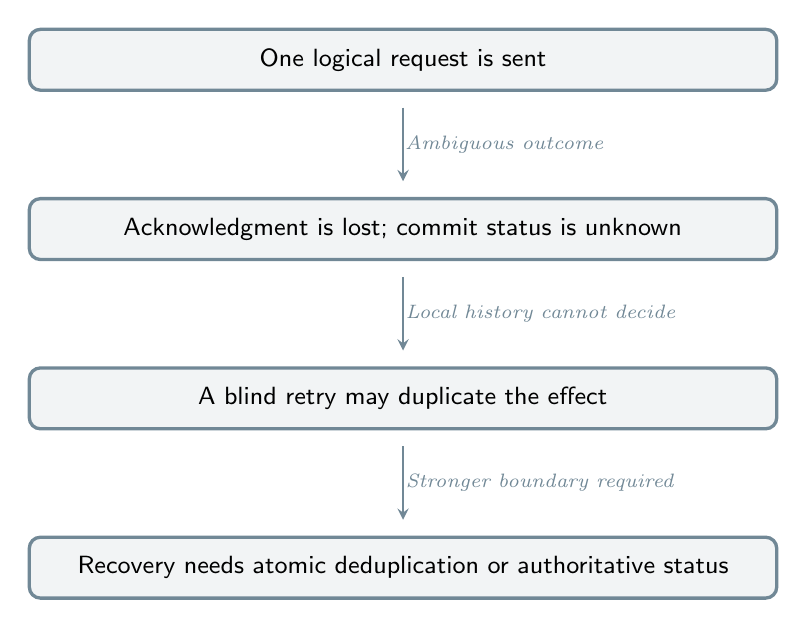
\begin{tikzpicture}[x=1cm,y=1cm,>=stealth,story node/.style={draw=blue!65,very thick,rounded corners=4pt,align=center,text width=9cm,font=\small\sffamily,fill=blue!6,inner sep=7pt}]
\node[story node] (request) at (0,0.00) {One logical request is sent};
\node[story node] (unknown) at (0,-2.15) {Acknowledgment is lost; commit status is unknown};
\node[story node] (retry) at (0,-4.30) {A blind retry may duplicate the effect};
\node[story node] (contract) at (0,-6.45) {Recovery needs atomic deduplication or authoritative status};
\draw[->,thick,blue!65,shorten <=2mm,shorten >=2mm] (request) -- node[midway,right,font=\scriptsize\itshape,align=left,text width=3.8cm,fill=white,inner sep=1pt] {Ambiguous outcome} (unknown);
\draw[->,thick,blue!65,shorten <=2mm,shorten >=2mm] (unknown) -- node[midway,right,font=\scriptsize\itshape,align=left,text width=3.8cm,fill=white,inner sep=1pt] {Local history cannot decide} (retry);
\draw[->,thick,blue!65,shorten <=2mm,shorten >=2mm] (retry) -- node[midway,right,font=\scriptsize\itshape,align=left,text width=3.8cm,fill=white,inner sep=1pt] {Stronger boundary required} (contract);
\end{tikzpicture}
\caption{An ambiguous acknowledgment leaves two externally different outcomes with the same local observation. A safe recovery claim therefore depends on a service contract that can prevent or identify a duplicate effect; the diagram is an analytical model, not a verified implementation.}
\par\smallskip{\scriptsize Source-linked claims: C8, C9, C10; evidence links appear in the claim notes.}
\end{figure}
\section{Atomic recovery contracts and crash semantics}
Atomic coupling of an external effect with its completion record supplies a conditional recovery contract: retries can preserve at-most-one effect without ensuring that an effect occurs or that the client learns of it. The workload considered here is a single intended ledger append with stable operation key $k$ and full payload $p$; the unit of analysis is that logical operation across its deliveries, retries, and crashes. The evaluator inspects the durable effect multiset $E$ directly and checks its correspondence with the completion map $D$, rather than treating a completion record as its own outcome oracle.

Correctness requires exactly one matching effect and no unintended effect at the declared observation horizon, whereas the safety argument concerns every finite execution prefix.

The effect boundary is deliberately narrow: the covered effect is the committed ledger row, not a payment, email, or other downstream consequence. Atomicity, serialization, crash durability, record retention, stable identity, and independent observation are premises of the model, not properties established for an inspected service. The resulting argument and crash traces are analytical specifications, not observed benchmark results or measured reliability improvements; their application to an implementation remains unresolved.

The zero-effect base case is essential. Initially, $E$ and $D$ are empty, so the operation has neither an effect nor a completed record; the argument does not begin from an arbitrary state containing an unrecorded effect. A completed entry $D[k]$ stores the full payload, result, and effect identifier, while retries preserve $k$ and $p$ even though each transport delivery receives a fresh identifier. In the proposed ledger schema, the effect table deliberately permits multiple rows with the same logical key, so duplicate prevention must follow from the handler rather than being assumed by the outcome representation.

Atomic processing has three branches. When $D[k]$ is absent, one durable transaction creates an effect and its matching completion record together; when the record contains the same full payload, processing returns the stored result and identifier without creating another effect. A different payload is rejected without an effect. Serialization or uniqueness conflicts must abort the entire competing transaction, including its effect insertion, and an ambiguous commit outcome must lead back to a fresh record lookup rather than being treated as a known rollback.

Let $N_k$ count committed effects for key $k$. The candidate invariant is stronger than merely $N_k\in\{0,1\}$: either the completion record is absent and $N_k=0$, or the record identifies exactly one effect with the matching key and payload. Starting from the empty state, the first successful absent-key transition creates the matching pair; replay and rejection preserve it, and a crash exposes either the complete before-state or the complete after-state. Transport transitions do not alter that pair. This inductive argument therefore supports per-key safety under the stated premises, rather than an unconditional guarantee about agent recovery.

Concurrency requires the record test to occur at the serialized processing point, not merely when a request is received. Two workers may both be ready, but the worker processed second must inspect the record created by the first and replay its result. In a transactional realization, a competing absent-key insertion must instead lose serialization or uniqueness arbitration and roll back its effect write. Thus receiving a request does not reserve permission to perform an effect, and an earlier observation of an absent record cannot authorize an independent later append.

Safety does not supply existence: dropping every request leaves $N_k=0$ while satisfying at-most-once safety. Exactly one effect additionally requires at least one matching request to complete processing, either creating the effect or observing its existing record. Verified client completion requires further conditions on response creation, response delivery, and durable recording of client completion. None of these eventual conditions alone establishes completion by a deadline; the service can preserve the effect invariant while the client remains unable to verify success within its execution budget.

Reproducible crash schedules also require an explicit request lifecycle. Partition the pending-envelope pool into requests $Q_R$ and acknowledgments $Q_A$, with volatile workers held in $V$. A request envelope $(x,k,p)$ has a fresh delivery identifier $x$ distinct from the stable operation key; its acknowledgment has a fresh envelope identifier and correlates its outcome with $x$. The envelope pool survives service crashes but permits explicit permanent drops, while delay leaves an envelope eligible for later processing. This is a destructive-dequeue model, not a broker model with automatic redelivery.

RECEIVE removes an envelope from $Q_R$ and transfers it exclusively into a ready worker in $V$. PROCESS evaluates the current completion record and converts that worker into a processed worker carrying the outcome; it does not yet create an acknowledgment envelope. ACK\_\allowbreak{}ENQUEUE subsequently creates the acknowledgment in $Q_A$ and removes the processed worker. CRASH clears volatile workers without reconstructing their consumed deliveries, while preserving durable effects, completion records, and envelopes still queued. The table makes the resulting boundaries explicit for one initially unperformed operation.

The effect-first counterexample separates these atomic requirements from a superficially similar two-write handler. The first delivered attempt checks an absent record, commits its effect, and crashes before writing completion; after restart, a second delivered attempt again sees no record and commits another effect. The resulting $N_k=2$ is a possible safety violation of this particular protocol, even with a stable key and unchanged payload. The counterexample requires the retry actually to be processed: issuing a retry alone does not create the second effect.

Marker-first handling fails differently. A naive handler can durably write a purported completed record containing a reserved effect identifier, crash before performing the effect, and then return cached success on retry despite $N_k=0$. A more conservative marker-first protocol can instead use a reservation gate: only its uniquely confirmed creator may attempt one append, retries encountering the gate return an unknown or suppressed outcome, and restart never resumes the append. Under those rules, a crash between reservation and append can permanently omit the effect while preserving at-most-once safety; the reservation is not evidence of completion.

The broader assertion that separating the writes necessarily destroys at-most-once safety must therefore be withdrawn. Effect-first duplication and marker-first omission are local counterexamples to different parts of the stronger effect-and-completion contract, not a refutation of every non-atomic recovery protocol. Atomic effect-and-record insertion remains a sufficient conditional design for preserving the covered outcome across retries, while explicit dequeue and acknowledgment semantics determine what recovery must still accomplish. The central argument consequently shifts from treating deduplication as completion to distinguishing preserved safety, actual effect existence, and verified deadline-bounded completion.

\begin{longtable}{@{}>{\raggedright\arraybackslash}p{\dimexpr(\linewidth-2\tabcolsep*3)/168*42\relax}>{\raggedright\arraybackslash}p{\dimexpr(\linewidth-2\tabcolsep*3)/168*42\relax}>{\raggedright\arraybackslash}p{\dimexpr(\linewidth-2\tabcolsep*3)/168*42\relax}>{\raggedright\arraybackslash}p{\dimexpr(\linewidth-2\tabcolsep*3)/168*42\relax}@{}}
\caption{Predicted crash-boundary states under destructive dequeue and atomic effect\textendash{}\allowbreak{}record insertion. Each row considers the original delivery for one initially unperformed operation, with no additional deliveries or explicit envelope drops. These are model-derived outcomes, not executed fault-injection results.}\\
\toprule
\textbf{Crash boundary} & \textbf{Durable effect and completion state} & \textbf{Original request after crash} & \textbf{Original acknowledgment after crash}\\
\midrule
\endfirsthead
\toprule
\textbf{Crash boundary} & \textbf{Durable effect and completion state} & \textbf{Original request after crash} & \textbf{Original acknowledgment after crash}\\
\midrule
\endhead
\midrule
\multicolumn{4}{r}{\footnotesize Continued on next page}\\
\endfoot
\bottomrule
\endlastfoot
Before RECEIVE & $N_k=0$; $D[k]$ absent & Remains in $Q_R$ and is eligible for later receipt & Not created\\
After RECEIVE, before PROCESS & $N_k=0$; $D[k]$ absent & Consumed delivery is lost with the ready worker; no automatic redelivery & Not created\\
After PROCESS commits, before ACK\_\allowbreak{}ENQUEUE & $N_k=1$; $D[k]$ identifies the matching effect & Consumed delivery is lost with the processed worker & Not created; the crash does not reconstruct it\\
After ACK\_\allowbreak{}ENQUEUE, before acknowledgment delivery & $N_k=1$; $D[k]$ identifies the matching effect & Processing and acknowledgment enqueueing are complete; no worker remains & Remains in $Q_A$, subject to subsequent delivery or explicit drop\\
\end{longtable}
\par\smallskip{\footnotesize Evidence: [Research session 4, artifact 2], [Research session 4, artifact 4]; claims: C10, C12}
\section{Retention, cancellation, and containment}
Retention and cancellation constrain recovery only when they prevent later effect-capable execution, rather than merely stop the agent from sending requests. The unit of analysis here is one logical operation with an immutable payload and stable identity, including its retries, queued copies, and resumed workers; the outcome oracle is its actual irreversible-effect count, denoted $C(t)$, rather than a completion response or the presence of a receipt. At-most-once safety requires $C(t)\leq 1$ at every execution prefix, including after an evaluation horizon $H$, whereas effect completion by that horizon requires $C(H)=1$.

The arguments below distinguish conditional safety contracts and constructed counterexamples from implementation evidence: no independently audited execution or real-service validation establishes the stipulated atomicity, timing, or universal execution gating, which would require observation of actual effects independently of receipts and client reports. [C13\textendash{}\allowbreak{}C15, C18, C19]

Finite receipt retention invalidates an unrestricted inference from stable identity and atomic effect-plus-receipt commitment to at-most-once execution. In the constructed schedule, the first effect commits at time $1$ and its receipt has retention duration $T=10$, so suppression expires at time $11$; an outstanding request bearing the same key executes at time $12$ and creates a second effect. The client can already have stopped issuing retries without preventing this duplication, because stopping issuance does not withdraw requests that remain capable of executing. Likewise, an ingress cutoff is insufficient if an accepted request can remain queued until after suppression expires.

The counterexample retracts the unrestricted finite-retention guarantee, not the conditional argument that applies when suppression covers every execution opportunity. Once a receipt expires, its absence is no longer evidence that the operation never committed. Thus, increasing confidence in client shutdown or preserving the original key does not address the decisive gap: the service must still distinguish an unperformed operation from a previously performed operation whose receipt has been removed, or reject execution without needing that distinction.

The first sufficient protection contract retains suppression through every possible effect-capable execution. If a first commitment occurs at time $c$ and its receipt expires at $c+T$, every later transition that could create another effect must occur strictly before $c+T$ and inspect the retained record under the stipulated serialized check-and-commit contract. The strict boundary matters because a transition at expiry cannot rely on a record that is no longer valid. Establishing this premise requires a bound on the last possible processing of every copy, including delayed, redelivered, and resumed requests; an average latency, client send cutoff, or ingress deadline does not establish that bound.

The second protection contract separates result retention from duplicate suppression. A durable tombstone installed atomically with commitment can continue to prohibit execution after the result itself expires; alternatively, an enforceable rejection boundary can eliminate later effect opportunities. The safety requirement concerns persistent suppression or rejection, not indefinite availability of the returned result. Neither protection contract guarantees that an effect occurs, that its result remains retrievable, or that completion is reported by a deadline.

Concurrent workers require a refinement of these protections because eligibility and receipt observations can become stale before commitment. In the supplied concurrent contract, every effect-producing path uses the same immutable authorization interval $[a,D)$, with $0<D-a\leq T$, and a first commitment at time $c$ creates a receipt valid on $[c,c+T)$ without renewal on replay. Current execution eligibility, current receipt inspection, and actual effect-plus-receipt commitment must share one per-operation ordering, with garbage collection respecting receipt validity. A worker\textquoteright{}s earlier observation that execution was eligible or that no receipt existed cannot substitute for these checks at the effect boundary.

The conditional safety argument then partitions every later effect attempt at the authorization deadline. Since the first commitment satisfies $c\geq a$, its suppression interval reaches at least the end of authorization: $c+T\geq a+T\geq D$. Any later attempt before $D$ must therefore encounter retained suppression, while an attempt at or after $D$ must be rejected by the execution-time eligibility check. When expiry equals the deadline, either ordering of garbage collection and an attempted execution is safe only because execution is already ineligible; a paused worker cannot carry a pre-deadline authorization check across that boundary. This strengthens the earlier serialized argument without making finite retention alone sufficient.

Cancellation provides a different certificate: under a stronger contract, it can establish that an initially unperformed operation has neither executed nor retained any future opportunity to execute. Let its durable state $S$ be PENDING, APPLIED, or CANCELLED, with the invariant that $S\in\{\mathrm{PENDING},\mathrm{CANCELLED}\}$ implies $C=0$, while $S=\mathrm{APPLIED}$ implies $C=1$. Cancellation and actual-effect commitment must compete as crash-atomic transitions out of PENDING, and every effect-producing path must obey this state gate. A durable CANCELLED acknowledgment then certifies both the absence of prior commitment and the exclusion of later gated effects.

The acknowledgment\textquoteright{}s meaning depends on which transition wins, not on which request the client sends first. If effect commitment wins, an ALREADY\_\allowbreak{}APPLIED response reports that outcome; it is not cancellation or rollback. If cancellation wins, queued and resumed workers must remain unable to commit, including after crashes or client recovery, so cancellation suppression must cover every later execution opportunity. Client stopping, a cached eligibility check, an acknowledgment issued before durable suppression, or cancellation state that expires while work remains executable cannot supply this certificate.

Post-incident closure has a deliberately weaker historical claim but can apply when cancellation\textquoteright{}s clean-state premise no longer holds. A durable CLOSED gate, checked atomically at every covered effect-creation boundary, conditionally prevents additional covered effects after closure commits and until authorized reopening, even when the historical effect count already exceeds one. Unlike cancellation from PENDING, closure need not certify that no prior effect occurred. Its contribution is to stop further growth of the covered effect history, not to restore an at-most-once property that has already been violated.

The containment boundary also limits what closure can repair or prevent. Historical committed effects remain part of the count even if refunds or corrective records are later created, and closure alone establishes neither successful compensation nor notification receipt. Already accepted downstream work remains outside the guarantee unless its eventual effect-creation path also enforces the gate. Consequently, the recovery argument must distinguish three achievements: preserving at-most-once execution through retention or rejection, certifying zero effects through competing cancellation, and containing additional effects through closure; none can be substituted for repairing historical harm.

\begin{longtable}{@{}>{\raggedright\arraybackslash}p{\dimexpr(\linewidth-2\tabcolsep*3)/168*42\relax}>{\raggedright\arraybackslash}p{\dimexpr(\linewidth-2\tabcolsep*3)/168*42\relax}>{\raggedright\arraybackslash}p{\dimexpr(\linewidth-2\tabcolsep*3)/168*42\relax}>{\raggedright\arraybackslash}p{\dimexpr(\linewidth-2\tabcolsep*3)/168*42\relax}@{}}
\caption{Conditional guarantees differ in their historical premises and temporal scope. These are analytical contracts, not measured implementation outcomes.}\\
\toprule
\textbf{Contract} & \textbf{Required starting condition} & \textbf{Certified effect property} & \textbf{What it does not establish}\\
\midrule
\endfirsthead
\toprule
\textbf{Contract} & \textbf{Required starting condition} & \textbf{Certified effect property} & \textbf{What it does not establish}\\
\midrule
\endhead
\midrule
\multicolumn{4}{r}{\footnotesize Continued on next page}\\
\endfoot
\bottomrule
\endlastfoot
Retention-protected or durably rejected execution & Initially unperformed operation; all effect paths obey the applicable atomic suppression and execution rules & At most one effect across execution prefixes, with protection extending through every effect-capable opportunity & Existence of an effect, result availability, or deadline completion\\
Durably acknowledged cancellation & Initially unperformed operation; cancellation and actual commitment compete from PENDING & Zero prior effects and no future gated effects after CANCELLED & Rollback when execution has already won\\
Durable closure & Historical effects may already exist, including duplication; all covered future effect transitions obey the closure gate & No additional covered effects after closure commits while the gate remains closed & Removal of historical duplication, compensation, notification receipt, or containment of ungated downstream work\\
\end{longtable}
\par\smallskip{\footnotesize Evidence: [Research session 6, artifact 4], [Research session 6, artifact 5], [Research session 6, artifact 7], [Research session 6, artifact 6], [Research session 7, artifact 7]; claims: C14, C15, C18, C19}
\section{Evidence contracts and truthful reporting}
A reliability certificate needs two distinct things: a mapper that follows its rules, and evidence that truthfully covers the execution. Consider one scheduled append operation in an isolated, initially empty namespace with expected payload $p$. Its history $w$ orders durable commits, accepted final-report receipts, and cutoff $H$. Let $E_H(w)=1$ only for exactly one covered append with $p$ before $H$, and let $R_H(w)=1$ only for exactly one timely, well-formed matching SUCCESS receipt. The horizon outcome is $Y_H=E_H\land R_H$; nonexecution remains a failed scheduled slot. These oracles are external to the agent's own report.

From routine evidence $d$ and authorization state $a$, the conservative mapper assigns nonempty component sets $U_E,U_R\subseteq\{0,1\}$ and returns $S=m(d,a)=\{e\land r:e\in U_E,\ r\in U_R\}$. A complete, usable certificate may determine a component by its full rubric. A sound irreversible-violation witness, such as two distinct commits, may establish failure without complete enumeration; one observed matching commit cannot establish uniqueness. Missing evidence gives $\{0,1\}$, and recognized contradictions or quarantined authorities widen affected components instead of yielding an empty set.

Four predicates keep the assurance claim precise. $M(d,a,S)$ means the mapper used the specified rule for the supplied evidence and authorization version; $V(d,w)$ means the certificate's content, completeness, namespace, and cutoff assertions are true; $Z(S,w)$ means the actual outcome $Y_H(w)$ belongs to $S$. A separate hold $B_t(D)$ suspends certification depending on trust domain $D$ while authorization, contradiction, or a disclosed breach remains unresolved. It neither proves task failure nor repairs false evidence. Under the stated contract, $V\land M$ implies $Z$: each actual component lies in its assigned set, so their conjunction lies in $S$.

The converse directions fail. A conforming mapper can return $\{1\}$ from a false complete certificate even when the actual outcome is $0$; valid evidence does not force a faulty mapper to conform, and containment can occur accidentally. The analytical table gives reconstructed examples, not observed incidents. Disclosure reveals that a silently false certificate was already invalid; it does not retroactively change the frozen mapper's conformance. Remediation preserves the original record, creates a new evidence version, quarantines affected authorities, and widens only components whose support was lost. A replacement mapping does not validate the old certificate or automatically lift the hold.

A randomized audit of a frozen paired roster can support conditional finite-roster coverage if the outcome sets are sound and audit selection is uniform, even when execution outcomes are correlated. Unknown labels can be widened conservatively; a falsely definite label that excludes truth breaks the premise. Such coverage is neither a posterior probability that a particular roster is correct nor a deployment-reliability estimate. Certificate soundness, observer completeness, audit compliance, and mapper conformance remain unvalidated here: no pilot or measured agent improvement is supplied.

Horizon success also differs from truth at report time. Let $X_h$ mean exactly one correct covered commit by cutoff $h$, let $Y_{\mathrm{window}}$ require horizon success and correctness at a later cutoff, and let $T$ require the full reporting contract and the unique correct effect immediately before report emission. In an analytical control, a matching SUCCESS at tick $15$ followed by the sole commit at tick $18$, with horizon $H=20$ and no extra commit through tick $40$, gives \[(X_{20},X_{40},Y_H,Y_{\mathrm{window}},T)=(1,1,1,1,0).\] Moving the commit to tick $14$ changes only the final entry to $1$. A correct end state therefore does not establish that the earlier completion claim was true.

Retained evidence can express this uncertainty without guessing. If $W(d)$ is the set of histories consistent with $d$, define $O_P(d)=\{P(w):w\in W(d)\}$ for predicate $P$; the actual history's value belongs to that set when the evidence contract is sound. Joint predicates must use the same histories. A singleton success label needs complete capture of report content, uniqueness, timing, and closure, not one matching row and one SUCCESS message. An INDETERMINATE, late SUCCESS, or multiple final reports fails the specified reporting contract even if the external effect is correct.

The evidence must genuinely permit any claimed ordering uncertainty. Trusted common-clock timestamps can still show that a report preceded commitment after a separate ordering certificate is removed; same-tick timestamps without within-tick order may leave both histories possible. The resulting assurance boundary is twofold: a conforming evaluator needs truthful evidence for containment, and a correct horizon state needs separate report-time adjudication for a truthful completion claim.

\begin{figure}[!htbp]
\centering
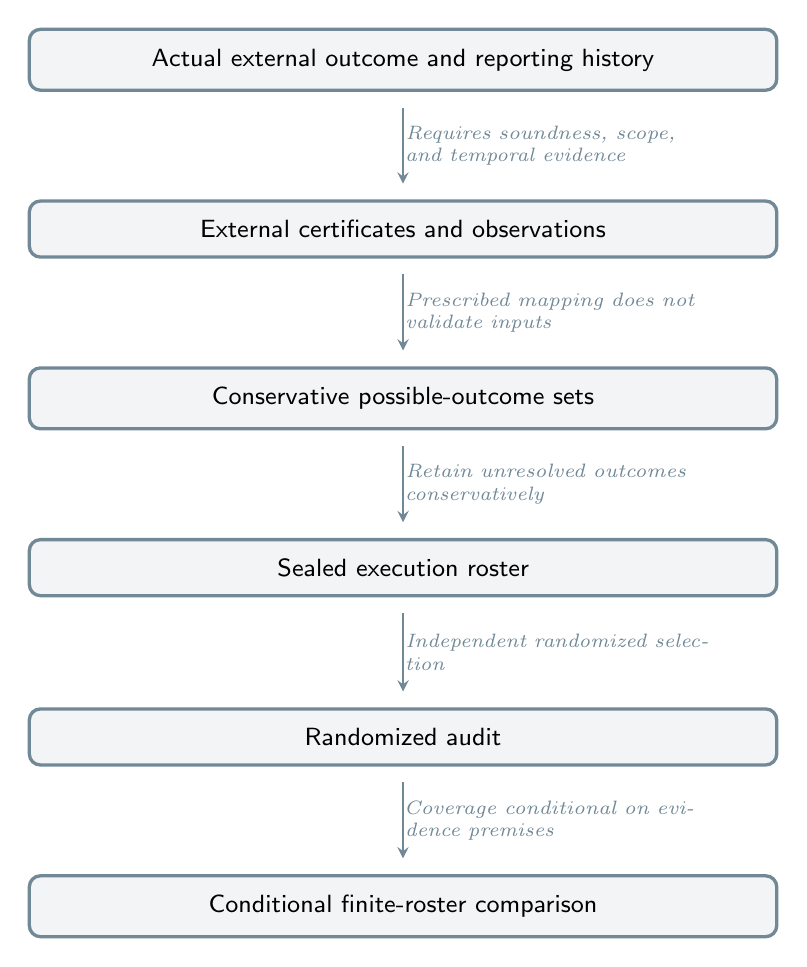
\begin{tikzpicture}[x=1cm,y=1cm,>=stealth,story node/.style={draw=blue!65,very thick,rounded corners=4pt,align=center,text width=9cm,font=\small\sffamily,fill=blue!6,inner sep=7pt}]
\node[story node] (outcome) at (0,0.00) {Actual external outcome and reporting history};
\node[story node] (evidence) at (0,-2.15) {External certificates and observations};
\node[story node] (mapper) at (0,-4.30) {Conservative possible-outcome sets};
\node[story node] (roster) at (0,-6.45) {Sealed execution roster};
\node[story node] (audit) at (0,-8.60) {Randomized audit};
\node[story node] (bound) at (0,-10.75) {Conditional finite-roster comparison};
\draw[->,thick,blue!65,shorten <=2mm,shorten >=2mm] (outcome) -- node[midway,right,font=\scriptsize\itshape,align=left,text width=3.8cm,fill=white,inner sep=1pt] {Requires soundness, scope, and temporal evidence} (evidence);
\draw[->,thick,blue!65,shorten <=2mm,shorten >=2mm] (evidence) -- node[midway,right,font=\scriptsize\itshape,align=left,text width=3.8cm,fill=white,inner sep=1pt] {Prescribed mapping does not validate inputs} (mapper);
\draw[->,thick,blue!65,shorten <=2mm,shorten >=2mm] (mapper) -- node[midway,right,font=\scriptsize\itshape,align=left,text width=3.8cm,fill=white,inner sep=1pt] {Retain unresolved outcomes conservatively} (roster);
\draw[->,thick,blue!65,shorten <=2mm,shorten >=2mm] (roster) -- node[midway,right,font=\scriptsize\itshape,align=left,text width=3.8cm,fill=white,inner sep=1pt] {Independent randomized selection} (audit);
\draw[->,thick,blue!65,shorten <=2mm,shorten >=2mm] (audit) -- node[midway,right,font=\scriptsize\itshape,align=left,text width=3.8cm,fill=white,inner sep=1pt] {Coverage conditional on evidence premises} (bound);
\end{tikzpicture}
\caption{The conditional evidence chain separates external outcomes, evidence validity, mapper conformance, and randomized auditing. None of these dependencies establishes that a practical implementation satisfies the required contract.}
\par\smallskip{\scriptsize Source-linked claims: C5, C6, C7, C20; evidence links appear in the claim notes.}
\end{figure}
\begin{landscape}
\small
\begin{longtable}{@{}>{\raggedright\arraybackslash}p{\dimexpr(\linewidth-2\tabcolsep*5)/167*23\relax}>{\raggedright\arraybackslash}p{\dimexpr(\linewidth-2\tabcolsep*5)/167*42\relax}>{\raggedright\arraybackslash}p{\dimexpr(\linewidth-2\tabcolsep*5)/167*20\relax}>{\raggedright\arraybackslash}p{\dimexpr(\linewidth-2\tabcolsep*5)/167*20\relax}>{\raggedright\arraybackslash}p{\dimexpr(\linewidth-2\tabcolsep*5)/167*20\relax}>{\raggedright\arraybackslash}p{\dimexpr(\linewidth-2\tabcolsep*5)/167*42\relax}@{}}
\caption{Conditional analytical fixtures separating mapper conformance, evidence validity, containment, and certification holds. Each fixture assumes an initially authorized issuer and a conforming mapper. The silently false fixtures are reconstructions, not observed incidents or identified historical cases. Hold decisions are shown before and after sound reference disclosure; the frozen mapping is unchanged.}\\
\toprule
\textbf{Fixture} & \textbf{Stipulated evidence and history} & \textbf{Frozen output $S$} & \textbf{Conformance $M$} & \textbf{Validity $V$} & \textbf{Containment $Z$ \textemdash{} $Y_H\in S$ implies the set contains truth, not necessarily success $Y_H=1$ in general; here shown directly as true or false \textemdash{} actual $Y_H$ noted in the history column where false evidence matters}\\
\midrule
\endfirsthead
\toprule
\textbf{Fixture} & \textbf{Stipulated evidence and history} & \textbf{Frozen output $S$} & \textbf{Conformance $M$} & \textbf{Validity $V$} & \textbf{Containment $Z$ \textemdash{} $Y_H\in S$ implies the set contains truth, not necessarily success $Y_H=1$ in general; here shown directly as true or false \textemdash{} actual $Y_H$ noted in the history column where false evidence matters}\\
\midrule
\endhead
\midrule
\multicolumn{6}{r}{\footnotesize Continued on next page}\\
\endfoot
\bottomrule
\endlastfoot
Clean evidence & Exactly one correct commit and one valid final receipt precede $H$; matching complete certificates. No hold before or after disclosure. & $\{1\}$ & True & True & True\\
Visible conflict & Certificates assert incompatible exact counts for the same namespace and cutoff. Hold before and after disclosure. & $\{0,1\}$ & True & False & True\\
Silent commit omission & Certificates assert a clean history, but omit a second pre-cutoff commit; actual $Y_H=0$. No hold before disclosure; hold afterward. & $\{1\}$ & True & False & False\\
Silent receipt omission & Certificates assert a clean history, but omit an additional pre-cutoff final receipt; actual $Y_H=0$. No hold before disclosure; hold afterward. & $\{1\}$ & True & False & False\\
\end{longtable}
\par\smallskip{\footnotesize Evidence: [Research session 7, artifact 9]; claims: C6}
\end{landscape}
\section{Discriminating evaluation and limits of assurance}
A discriminating evaluation must test the correctness of its observations and injected faults before attributing outcome differences to an agent or recovery mechanism. The proposed sequence therefore begins with independent oracle and injector validation, proceeds through deterministic boundary schedules and service-contract audits, and only then compares agent policies under controlled conditions. This ordering makes the analytical assumptions testable rather than treating them as established properties of an implementation.

The evaluation protocol should first freeze the workload, outcome rubric, unit of analysis, evaluators, and execution horizon. For the narrow external-effect workload, one logical debit request is evaluated by its authoritative effect count at the specified horizon $H$; exactly one applied debit satisfies the effect-count requirement, while acknowledgment receipt is recorded separately. Broader task success must additionally use prespecified end-state, safety, and deadline requirements.

Repeated executions should be organized into task clusters, with automated acceptance and independent outcome adjudication retained for each audited execution; crashes and timeouts remain attempted executions rather than disappearing from the denominator. [C31; [Research session 1]]

The supplied boundary schedules and conformance panels are analytical test specifications, not executed experiments. They establish neither implementation conformance nor observed agent failure rates, recovery benefits, or causal architectural improvements. Moreover, incomplete historical extracts and unavailable originals restrict the contribution to a scoped synthesis: omitted objections cannot be treated as resolved, and the supplied material does not constitute an exhaustive literature or benchmark assessment. [C20, C21; [Research session 7, artifact 6]]

The first implementation stage should independently test both the ledger oracle and the fault injector, especially their ability to distinguish a failure before commitment from acknowledgment loss after commitment. Final-state reads must be checked for freshness and noninterference, rather than assumed to reveal authoritative state without changing the task. The reference observer also needs a concrete capture-and-cutoff protocol covering durable effects, ingress receipts, isolation, and crash boundaries.

Independent retention is insufficient unless the observer actually captures every relevant event; agreement between the agent's evaluator and a reference judge cannot establish the rate of jointly accepted failures, so unsupported reference-error allowances must remain sensitivity parameters rather than reported calibration. [C30, C23; [Research session 1]; [Research session 7, artifact 6]]

Deterministic execution should then precede stochastic agent evaluation. The proposed seven path checks, six-case boundary experiment, and seventeen-case evidence panel address different obligations and should retain separate verdicts. Their execution should cover receipt/effect crash boundaries, stable versus regenerated operation keys, delayed effects, missing evidence, visible contradictions, and silently false certificates, while keeping routine evidence separate from held-out reference evidence.

Results should distinguish mapper conformance, service or controller contract failures, and failures of actual-outcome containment; otherwise a correctly implemented mapper operating on false evidence could be misdiagnosed as an implementation defect. [C30, C20; [Research session 1]; [Research session 5]; [Research session 7, artifact 6]]

A real-service audit is a separate applicability requirement, not a consequence of passing synthetic schedules. Before applying the atomic stable-key argument, the audit should establish effect/receipt atomicity, key namespace and lifetime, payload consistency, concurrent-call behavior, retention and expiry, response semantics, and downstream effects. Crash, failover, and restore checks should test whether the relevant durability guarantees survive the failures against which recovery is claimed. Where revocation or settlement progress is required, those properties likewise need direct validation rather than inference from the existence of an idempotency interface. [C85; [Research session 5]]

Only after these checks should the study conduct paired policy comparisons, fixing task definitions and weights, model and prompt versions, tool contracts, environment generation, deadlines, and resource budgets. Candidate comparisons include bounded retry, status reconciliation, safe escalation, restart, and reconciliation, but the analytical traces do not select a preferred policy. Shared fault schedules should be distinguished from mechanism-specific outage tests, and paired executions require isolation sufficient to prevent one policy's external effects from changing the other's task.

Sample sizes or precision targets and paired uncertainty estimates should be preregistered, with token, tool, latency, and monetary budgets reported separately because invocation count alone is not total cost. [C31; [Research session 1]; [Research session 5]]

The sampling design must preserve the distinction between independent task clusters and correlated repetitions of the same task. Repetition can characterize within-task variability, but it should not be counted as additional independent task sampling; cluster independence, population matching, and noninterference require evidence in the implemented evaluation. A finite-roster audit should separately validate roster completeness, randomized selection, evidence mapping, and bound calculation, including all-unknown evidence and outcome-dependent evidence loss.

Missing or inconsistent audits must remain unresolved under prespecified conservative treatment, while failed attempts, seeds, versions, tool traces, adjudications, and resource records should be retained rather than selected out of the comparison. [C31, C30; [Research session 1]; [Research session 5]; [Research session 7, artifact 6]]

Stress testing should explicitly vary correlated and persistent failures, delayed acknowledgments, transport duplication, concurrency, and deadline sensitivity rather than assume that an independent-attempt result transfers. Comparative outcomes should include regressions, severity, safe stopping, recovery quality, persistent-state corruption, delayed harm, and resource use alongside fixed-horizon success. Held-out task families and changed environments require separate evidence, as do multi-service workflows and settlement after $H$: exactly one effect for one logical operation does not establish end-to-end task correctness.

These measurements would determine whether a recovery mechanism improves the intended outcome under matched conditions, rather than merely increasing acknowledged completion. [C31, C85; [Research session 1]; [Research session 5]]

This evaluation sequence changes the assurance claim from an architectural expectation into a set of separable, falsifiable obligations. Conditional analysis identifies which observation and service premises would support a guarantee; deterministic tests can challenge an implementation's compliance with those premises; outcome-grounded, controlled comparisons are needed to establish an improvement. Demonstrated deployment reliability would additionally require justified sampling and transport to the relevant tasks, environments, versions, and budgets\textemdash{}not merely successful execution of the boundary schedules.

\begin{table}[!htbp]
\centering\small
\caption{Proposed evaluation stages and the distinct assurance question each addresses. These are validation requirements, not completed tests or observed results.}
\begin{tabular}{@{}>{\raggedright\arraybackslash}p{\dimexpr(\linewidth-2\tabcolsep*2)/116*32\relax}>{\raggedright\arraybackslash}p{\dimexpr(\linewidth-2\tabcolsep*2)/116*42\relax}>{\raggedright\arraybackslash}p{\dimexpr(\linewidth-2\tabcolsep*2)/116*42\relax}@{}}
\toprule
\textbf{Stage} & \textbf{Required discriminating checks} & \textbf{Conclusion not warranted by this stage alone}\\
\midrule
Oracle and injector validation & Distinguish precommit failure from postcommit acknowledgment loss; test fresh, nonmutating state reads and complete reference capture. & Evaluator agreement does not establish actual correctness or calibrate shared reference errors.\\
Deterministic boundary execution & Run the proposed path, recovery, and evidence panels; separately classify mapper, contract, and containment failures. & Passing finite cases does not prove universal coverage or a measured agent-level benefit.\\
Real-service contract audit & Check atomicity, key scope, payload binding, concurrency, retention, response semantics, durability, and downstream effects. & Synthetic conformance does not establish that an external service satisfies the recovery premises.\\
Controlled paired comparison & Freeze workload, versions, environment, rubric, horizon, and budgets; retain failures and unknowns; report paired uncertainty and broader harms. & A fixed-protocol comparison does not automatically transfer to changed tasks, environments, versions, or budgets.\\
\bottomrule
\end{tabular}
\par\smallskip{\scriptsize Source-linked claims: C20, C23, C30, C31, C85}
\end{table}
\section{Limitations}
\begin{itemize}
\item The analytical guarantees depend on unvalidated reference-error, evidence-soundness, atomicity, durability, identity, retention, and enforcement-scope premises.
\item No implementation, benchmark audit, controlled agent comparison, or empirical cost analysis was completed.
\item The irreversible-effect workload does not establish general reliability across open-ended agent tasks.
\item The evidence selection is bounded and includes incomplete historical arguments.
\item Saved research session a1a9ab51-f8d1-4b60-ba10-baad7585a34f ended with an incomplete review; call 8 (investigator) was not successfully completed. Earlier findings remain available, but this process limitation prevents claiming that the planned adversarial review was fully performed.
\item Saved research session ebc7ac05-823c-4a02-9590-1e9f9726e807 ended with an incomplete review; a research review was not successfully completed. Earlier findings remain available, but this process limitation prevents claiming that the planned adversarial review was fully performed.
\item Saved research session e3f02cce-aed5-42f7-aa01-a5cad3c99c18 ended with an incomplete review; call 19 (skeptic) was not successfully completed. Earlier findings remain available, but this process limitation prevents claiming that the planned adversarial review was fully performed.
\end{itemize}
\section{Open obligations}
\begin{itemize}
\item Recover complete proof notes and unresolved original objections before claiming historical compatibility or validated proofs.
\item Validate directional reference-error allowances against justified external outcome evidence.
\item Implement and independently test the authoritative outcome oracle and fault injector.
\item Execute the crash, delayed-request, expiry, concurrency, cancellation, and false-certificate controls.
\item Audit real-service atomicity, key scope, payload checks, retention, downstream effects, and acknowledgment semantics.
\item Conduct controlled paired comparisons and report correctness, uncertainty, latency, resource consumption, and monetary cost without discarding unresolved executions.
\end{itemize}
\section{Conclusions}
Reliability evaluation must distinguish actual outcomes, reported completion, and the evidence used to certify each. Conditional statistical guarantees can accommodate correlated repetitions and imperfect judges, but their remaining truth-error assumptions require external validation.

Safe recovery depends on enforceable service contracts at the actual effect boundary. Stable keys, checkpoints, negative reads, and client stopping are not interchangeable with atomic suppression or durable execution-time cancellation.

The supported contribution is an analytical framework and proposed validation program. Demonstrated architectural benefit and deployment reliability remain open empirical questions.

\appendix
\section{Claim and source notes}
These notes identify the saved evidence for claims used in the article. The complete claim register and reasoning are retained in the paper record.
\begin{sloppypar}
\small
\begin{description}
\item[C15] Under the stated concurrent finite-retention contract, at-most-once safety survives overlapping workers and receipt garbage collection when current eligibility, receipt inspection, and effect-plus-receipt commitment share one per-operation ordering. For authorization interval $[a,D)$ with $D-a\leq T$, a first commitment at $c\geq a$ has suppression lasting through the remaining eligible interval because $c+T\geq D$. \textit{Status: }unresolved.
\textit{Evidence: }[Research session 6, artifact 7]
\item[C16] A negative linearizable status read does not make replacement safe when an outstanding original request can still execute. The legal ordering $\operatorname{status}(r)<\operatorname{commit}(r')<\operatorname{commit}(r)$ produces two effects even though the negative read was accurate when performed. \textit{Status: }established.
\textit{Evidence: }[Research session 8, artifact 4], [Research session 7, artifact 2]
\item[C17] Under the specified delayed-or-discarded execution model, wrapper-local records, epochs, clocks, and absence replies cannot provide both sound conclusive cancellation and eventual authorization of replacement if the downstream effect remains outside the wrapper's enforcement boundary. \textit{Status: }unresolved.
\textit{Evidence: }[Research session 8, artifact 5]
\item[C18] For an initially unperformed operation, a durable cancellation acknowledgment certifies no prior or future effect if cancellation and actual effect commitment are competing crash-atomic transitions from a pending state, every effect-producing path obeys that gate, and suppression covers every later execution opportunity. \textit{Status: }unresolved.
\textit{Evidence: }[Research session 6, artifact 6]
\item[C19] An atomic durable closure gate prevents additional covered effects after closure commits, even when historical effects already exist. It does not remove prior duplication, establish compensation, prove notification receipt, or contain already accepted downstream work outside the enforced boundary. \textit{Status: }unresolved.
\textit{Evidence: }[Research session 7, artifact 7]
\item[C20] The saved boundary schedules and fault-injection panels are proposed analytical tests, not executed experiments. The supplied evidence establishes no implemented harness conformance, observed agent failure rate, measured recovery benefit, or causal architecture improvement. \textit{Status: }limitation.
\textit{Evidence: }[Research session 1], [Research session 5], [Research session 7, artifact 6], [Research session 6, artifact 5]
\item[C21] The available evidence is a bounded selection containing incomplete historical extracts and unresolved continuity obligations. It supports a scoped analytical synthesis, not an exhaustive literature assessment or a claim that all earlier objections have been resolved. \textit{Status: }limitation.
\textit{Evidence: }[Research session 2], [Research session 3], [Research session 8], [Research session 7, artifact 9]
\item[C22] Subtracting two lower confidence bounds on individual reliability does not establish a lower bound on improvement. A valid improvement argument must also control how much baseline correctness can exceed its observed or certified surrogate. \textit{Status: }established.
\textit{Evidence: }[Research session 5, artifact 1], [Research session 5, artifact 3]
\item[C23] Agreement between the agent's evaluator and a reference judge does not establish a useful bound on jointly accepted failures. Without justified external outcome evidence, reference-error allowances must be reported as sensitivity parameters rather than measured calibration. \textit{Status: }limitation.
\textit{Evidence: }[Research session 4, artifact 1], [Research session 2], [Research session 3]
\item[C13] Stable operation identity and atomic effect-plus-receipt commitment do not ensure at-most-once effects after suppression expires. In the saved constructed schedule, an effect commits at time $1$, a retention duration of $10$ expires at time $11$, and an outstanding same-key request executes at time $12$, creating another effect. \textit{Status: }established.
\textit{Evidence: }[Research session 6, artifact 4], [Research session 6, artifact 5]
\item[C14] Two stated contracts suffice to restore at-most-once safety with finite result retention: suppression that remains effective through every possible effect-capable execution, or durable rejection state that survives result expiry and blocks later execution. These are safety conditions, not guarantees that an effect will occur. \textit{Status: }unresolved.
\textit{Evidence: }[Research session 6, artifact 4], [Research session 6, artifact 5]
\item[C12] In the refined destructive-dequeue model, receiving a request removes its delivery envelope from the durable queue and places execution only in volatile worker state. A crash loses that consumed worker without reconstructing its delivery, while envelopes still queued survive; commitment and acknowledgment enqueueing are separate transitions. \textit{Status: }established.
\textit{Evidence: }[Research session 4, artifact 4]
\item[C11] Effect-first and marker-first split-write handlers fail in different ways. Effect-first commitment followed by a crash before recording completion permits duplication on retry; marker-first suppression can retain at-most-once safety while omitting the effect and potentially returning a cached success. \textit{Status: }established.
\textit{Evidence: }[Research session 7, artifact 3], [Research session 7, artifact 5], [Research session 6, artifact 3]
\item[C10] For an initially unperformed logical operation, a stable key and serialized, durable, atomic effect-and-completion-record insertion preserve at-most-one covered effect through retries and crashes. Exactly one effect additionally requires a valid request to commit; eventual verified client completion also requires suitable response delivery and durable client completion. \textit{Status: }unresolved.
\textit{Evidence: }[Research session 4, artifact 2], [Research session 4, artifact 3], [Research session 6, artifact 2]
\item[C85] A real-service application of the atomic stable-key argument requires checking effect/receipt atomicity, key scope, payload consistency, concurrency, retention, response semantics, and downstream effects. \textit{Status: }unresolved.
\textit{Evidence: }[Research session 5]
\item[C31] The intended experiment compares outcomes under fixed task, model, prompt, tool, environment, budget, rubric, and horizon definitions. \textit{Status: }unresolved.
\textit{Evidence: }[Research session 1, artifact 1], [Research session 8, artifact 1]
\item[C30] The practical test program must first establish oracle and fault-injector correctness before using their outputs to compare agents. \textit{Status: }unresolved.
\textit{Evidence: }[Research session 1]
\item[C9] Relaxing guaranteed retry commitment invalidates the original retry-probability bound. \textit{Status: }established.
\textit{Evidence: }[Research session 5]
\item[C1] Reliability concerns actual rubric satisfaction under a fixed execution protocol, not completion reports alone. \textit{Status: }established.
\textit{Evidence: }[Research session 1, artifact 1]
\item[C2] If jointly accepted failures have probability at most $\eta$, then $p\geq\max(0,\Pr(O=1)-\Pr(O=1,R=0)-\eta)$. \textit{Status: }unresolved.
\textit{Evidence: }[Research session 4, artifact 1]
\item[C3] Repeated runs need not be independent; task-cluster sampling determines the stated concentration guarantee. \textit{Status: }unresolved.
\textit{Evidence: }[Research session 1, artifact 1]
\item[C4] Paired improvement bounds require directional truth-error corrections for candidate false successes and baseline missed successes. \textit{Status: }unresolved.
\textit{Evidence: }[Research session 5, artifact 3]
\item[C5] Random auditing can conditionally certify a frozen paired roster without independent execution outcomes. \textit{Status: }unresolved.
\textit{Evidence: }[Research session 6, artifact 1]
\item[C6] Mapper conformance, evidence validity, and actual-outcome containment are distinct properties. \textit{Status: }unresolved.
\textit{Evidence: }[Research session 7, artifact 9]
\item[C7] A success report at tick $15$ followed by the sole correct commit at tick $18$ can pass a horizon-$20$ end-state rubric while being false when emitted. \textit{Status: }established.
\textit{Evidence: }[Research session 7, artifact 8]
\item[C8] Under forced stop-or-retry recovery with guaranteed retry commitment, indistinguishable committed and uncommitted histories imply worst-case error at least $1/2$. \textit{Status: }unresolved.
\textit{Evidence: }[Research session 1, artifact 2]
\end{description}
\end{sloppypar}
\end{document}
